% Submission 1 presentation, Quantinuum Singapore Grand Challenge, team Learned ZX Rewriting.
% Content and numbers are taken only from value/policy_compare.md, value/psel4_zx_only.md,
% value/mechanism_zx_l3.md, value/zx_classifier.md, results/h22e_multi.md, results/h22e_famC_nz.md,
% results/h22e_confirmatory.md, results/family_C_equivalence_L3.md, results/strong_baselines.md,
% results/EVIDENCE.md and report/report_v5.md. Story: three findings (cost, mechanism, cost is not fidelity).
% Build: pdflatex presentation.tex (twice).
\documentclass[aspectratio=169,11pt]{beamer}
\usepackage[utf8]{inputenc}
\usepackage{booktabs}
\usepackage{tikz}
\usetikzlibrary{arrows.meta,positioning}

\usetheme{default}
\usefonttheme{professionalfonts}
\setbeamertemplate{navigation symbols}{}
\definecolor{ink}{HTML}{1F2933}
\definecolor{accent}{HTML}{1D5FA8}
\definecolor{opinion}{HTML}{8A4B08}
\definecolor{opbg}{HTML}{FFF4E5}
\definecolor{muted}{HTML}{5F6B76}
\setbeamercolor{normal text}{fg=ink,bg=white}
\setbeamercolor{frametitle}{fg=accent,bg=white}
\setbeamercolor{title}{fg=accent}
\setbeamercolor{itemize item}{fg=accent}
\setbeamercolor{itemize subitem}{fg=accent}
\setbeamerfont{frametitle}{size=\large,series=\bfseries}
\setbeamertemplate{itemize items}[circle]
\setbeamertemplate{frametitle}{\vspace*{2pt}\insertframetitle\par\vspace{-3pt}{\color{accent!40}\rule{\textwidth}{0.6pt}}}
\setbeamertemplate{footline}{%
  \hspace{0.55cm}{\color{muted}\footnotesize Untagged statements are [F] facts. [O] marks a judgement.}%
  \hfill{\color{muted}\footnotesize\insertframenumber}\hspace{0.55cm}\vspace{0.15cm}}
\setlength{\leftmargini}{1.1em}
\setbeamersize{text margin left=0.55cm,text margin right=0.55cm}
\setlength{\tabcolsep}{4pt}

% Judgement line, visually distinct from facts.
\newcommand{\assess}[1]{%
  \par\medskip\noindent\colorbox{opbg}{\parbox{\dimexpr\linewidth-2\fboxsep}{\small\color{opinion}\textbf{Assessment [O].} #1}}\par}
\newcommand{\Otag}{{\color{opinion}\textbf{[O]}}}
\newcommand{\code}[1]{\texttt{#1}}

\begin{document}

% ---------------------------------------------------------------- 1
\begin{frame}[plain]
  \vfill
  {\color{accent}\LARGE\bfseries PSEL4 compiles each H2 circuit four ways and keeps the cheapest\par}
  \vspace{0.45cm}
  {\large Over 217 benchmark circuits PSEL4 needs 15.7\,\% less HQC than pytket-quantinuum's default level 2. It costs more than level 2 on no circuit and never more than level 3.\par}
  \vspace{0.3cm}
  {\color{muted}Most of the saving comes from choosing level 3 where it is cheaper. On the H2-2E emulator the cheaper compile of cdkm\_adder\_10 returns the correct sum less often. [O] The finals goal is a selector that also learns fidelity.\par}
  \vspace{0.55cm}
  {\large Team Learned ZX Rewriting\par}
  \vspace{0.2cm}
  C.-F. Kam, A. Mahasinghe, D. De Silva, N. Karunarathne, F. Cadet, M. Bessafi, K. De Silva\par
  \vspace{0.45cm}
  {\color{muted}Quantinuum Singapore Grand Challenge, Submission 1\par
  October 2026\par}
  \vfill
\end{frame}

% ---------------------------------------------------------------- 2
\begin{frame}{The default compile of pytket-quantinuum is not the cheapest on H2}
  \small
  A run on Quantinuum H2 is billed in HQC.
  \[ \mathrm{HQC} = 5 + C\,\bigl(N_{1q} + 10\,N_{2q} + 5\,N_{\mathrm{SPAM}}\bigr) / 5000 \]
  {\footnotesize\color{muted} $C$ is the shot count. $N_{1q}$ counts PhasedX gates. $N_{2q}$ counts ZZPhase and ZZMax gates. $N_{\mathrm{SPAM}}$ counts initialisations, measurements and resets. Rz gates are free.\par}
  \smallskip
  \begin{itemize}\setlength{\itemsep}{2pt}
    \item pytket-quantinuum compiles at optimisation level 2 by default. Level 3 adds GreedyPauliSimp, a two-qubit resynthesis.
    \item Always using level 3 saves 13.9\,\% HQC over 217 circuits, yet it costs more than level 2 on 45 of them.
    \item ZX rewriting (PyZX teleport\_reduce) before the Quantinuum pass lowers the cost on some circuits and raises it on others.
    \item Qiskit at optimisation level 3, rebased to H2, costs 25.24\,\% more than level 2 on B1 and 25.16\,\% more on family C.
    \item \Otag\ A team with a fixed HQC budget cannot tell in advance which compile is cheapest for a given circuit.
  \end{itemize}
\end{frame}

% ---------------------------------------------------------------- 3
\begin{frame}{PSEL4 keeps the lowest HQC of four checked compilations}
  \small
  \begin{columns}[T,onlytextwidth]
    \begin{column}{0.56\textwidth}
      \begin{itemize}\setlength{\itemsep}{2pt}
        \item \textbf{L2 (P0).} pytket-quantinuum 0.59.3 at level 2, the default.
        \item \textbf{L3.} The same pass at optimisation level 3.
        \item \textbf{P2 and P2L3.} PyZX teleport\_reduce, then level 2 or level 3.
        \item \textbf{Exactness check.} Full unitary up to 8 qubits, all-zero input state from 9 to 20 qubits. Failed candidates are dropped.
        \item \textbf{Guarantee.} Level 2 and level 3 are always candidates. PSEL4 never costs more HQC than either where both pass the check. This holds by construction.
      \end{itemize}
    \end{column}
    \begin{column}{0.41\textwidth}
      \centering
      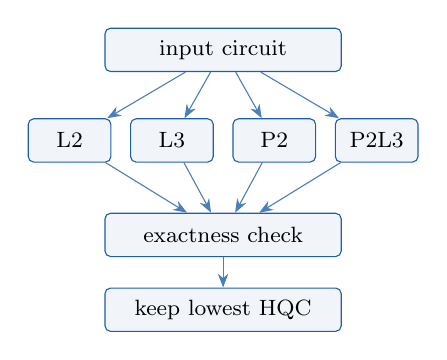
\begin{tikzpicture}[
          box/.style={draw=accent,rounded corners=2pt,fill=accent!6,minimum height=0.55cm,align=center,font=\footnotesize},
          arr/.style={-{Stealth[length=5pt]},color=accent!80}]
        \node[box,minimum width=3.0cm] (in) at (0,0) {input circuit};
        \node[box,minimum width=1.05cm] (p0) at (-1.95,-1.15) {L2};
        \node[box,minimum width=1.05cm] (l3) at (-0.65,-1.15) {L3};
        \node[box,minimum width=1.05cm] (p2) at (0.65,-1.15) {P2};
        \node[box,minimum width=1.05cm] (p2l3) at (1.95,-1.15) {P2L3};
        \node[box,minimum width=3.0cm] (chk) at (0,-2.35) {exactness check};
        \node[box,minimum width=3.0cm] (sel) at (0,-3.3) {keep lowest HQC};
        \foreach \n in {p0,l3,p2,p2l3} {\draw[arr] (in) -- (\n); \draw[arr] (\n) -- (chk);}
        \draw[arr] (chk) -- (sel);
      \end{tikzpicture}
      \par\vspace{2pt}{\footnotesize\color{muted}\code{pipelines/pass\_select.py --psel4}}
    \end{column}
  \end{columns}
  \assess{PSEL4 is pytket's PassSelector pattern with HQC as the metric. The contribution is the measured cost ledger, the correctness evidence and the emulator tests.}
\end{frame}

% ---------------------------------------------------------------- 4
\begin{frame}{Finding 1. PSEL4 needs 15.7\,\% less HQC than always using level 2}
  \footnotesize
  \centering
  \begin{tabular}{@{}lrrrrrrr@{}}
    \toprule
    & & \multicolumn{3}{c}{Total HQC} & \multicolumn{2}{c}{Saved vs always L2 \%} & \\
    \cmidrule(lr){3-5}\cmidrule(lr){6-7}
    Family & Circuits & Always L2 & Always L3 & PSEL4 & Always L3 & PSEL4 & L3 loses on \\
    \midrule
    A, Trotter & 180 & 16,422.6 & 16,231.2 & 15,949.0 & 1.2 & 2.9 & 35 \\
    B1, Clifford+T & 15 & 15,516.0 & 13,965.8 & 13,863.4 & 10.0 & 10.7 & 2 \\
    C, arithmetic and oracles & 20 & 24,535.0 & 18,853.2 & 18,193.2 & 23.2 & 25.8 & 8 \\
    Grover use case & 2 & 2,363.6 & 1,582.0 & 1,575.0 & 33.1 & 33.4 & 0 \\
    \midrule
    \textbf{Pooled} & \textbf{217} & 58,837.2 & 50,632.2 & 49,580.6 & 13.9 & \textbf{15.7} & \textbf{45} \\
    \bottomrule
  \end{tabular}
  \par\smallskip
  {\color{muted}HQC at 1000 shots. PSEL4 costs more than level 2 on 0 of 217 circuits. Source \code{value/policy\_compare.md}.\par}
  \par\smallskip
  \raggedright\footnotesize
  \begin{itemize}\setlength{\itemsep}{0pt}
    \item Always using level 3 loses 372.0 HQC on 45 circuits. The largest loss is 12.95\,\% on gf2\_pow\_4\_mult.
    \item PSEL4 saves 1,051.6 HQC more than always using level 3, or 1.79\,\% of the level 2 total.
    \item PSEL4 runs four compilations. Its total wall time is 5.08 times that of level 2 over 215 timed circuits. It saves 3.03 HQC per extra second.
  \end{itemize}
  \par\vspace{-4pt}\assess{For a cost-bound H2 user PSEL4 is a drop-in that cuts HQC by 15.7\,\% on this benchmark at about 5 times the compile time of level 2.}
\end{frame}

% ---------------------------------------------------------------- 5
\begin{frame}{Most level 3 and PSEL4 outputs are proven equal to their input}
  \small
  \centering\footnotesize
  \begin{tabular}{@{}lrlr@{}}
    \toprule
    Family C output & Proven & Not proven & Saved vs L2 (proven) \\
    \midrule
    Level 3 & 18 of 20 & hrs\_mult\_5, rgqft\_mult\_6 & 13.33\,\% \\
    PSEL4 & 17 of 20 & hrs\_mult\_5, rgqft\_mult\_6, draper\_adder\_28 & 10.22\,\% \\
    \bottomrule
  \end{tabular}
  \par\smallskip
  {\color{muted}Family C has 20 to 56 qubits. A PyZX miter reduction proves equality of the full unitary up to global phase. The level 3 miters of the two unproven circuits timed out after 900 s. Sources \code{results/family\_C\_equivalence\_L3.md}, \code{value/psel4\_zx\_only.md}.\par}
  \raggedright\footnotesize
  \begin{itemize}\setlength{\itemsep}{1pt}
    \item hrs\_mult\_5 has off-grid angles. Its PSEL4 output passes a check on 64 random basis inputs only. The PSEL4 miters of rgqft\_mult\_6 and draper\_adder\_28 timed out after 300 s.
    \item On families A, B1 and B2 every compiled circuit is checked against the uncompiled reference with tolerance 1e-8. All 1260 A rows, 105 B1 rows and 100 B2 rows pass.
    \item Our level 2 pipelines give the same counts and HQC as the official pytket-quantinuum pass on all 445 compiled rows of families A, B1, B1x and B2. Family C was not compiled with the official pass.
  \end{itemize}
\end{frame}

% ---------------------------------------------------------------- 6
\begin{frame}{Finding 2. Level 3 cuts two-qubit gates and ZX cuts phases}
  \footnotesize
  \centering
  \begin{tabular}{@{}lrrrrrrrr@{}}
    \toprule
    & \multicolumn{4}{c}{Non-Clifford gates} & \multicolumn{4}{c}{Two-qubit gates} \\
    \cmidrule(lr){2-5}\cmidrule(l){6-9}
    Set & L2 & P2 & L3 & P2L3 & L2 & P2 & L3 & P2L3 \\
    \midrule
    B1, 14 circuits & 877 & 656 & 746 & 701 & 862 & 799 & 723 & 700 \\
    C, 15 circuits & 3323 & 2930 & 2540 & 2535 & 3208 & 2944 & 2718 & 2708 \\
    \bottomrule
  \end{tabular}
  \par\smallskip
  {\color{muted}Totals after each pipeline. Source \code{value/mechanism\_zx\_l3.md}. 6 circuits are missing (compile budget).\par}
  \raggedright\small
  \begin{itemize}\setlength{\itemsep}{0pt}
    \item GreedyPauliSimp lowers the two-qubit count in level 3 on 180 of 180 A, 13 of 14 B1 and 9 of 15 C circuits.
    \item On B1 teleport\_reduce leaves fewer non-Clifford gates than level 3 (656 against 746). This rarely lowers HQC because a two-qubit gate costs 2 HQC at 1000 shots and a PhasedX 0.2.
    \item The ZX-only gain on top of the cheaper pytket level is 0.26\,\% on the 17 proven C circuits, 3.21\,\% on all 20, 0.49\,\% on B1 and 0 on the Trotter circuits.
    \item It falls as T-density rises (family C Spearman $\rho = -0.64$, $p = 0.010$).
  \end{itemize}
  \assess{The hypothesis that level 3 absorbs the ZX gain partly holds. It holds for two-qubit gates and fails for phase merging on B1.}
\end{frame}

% ---------------------------------------------------------------- 7
\begin{frame}{Finding 3. The cheaper compile is not always the more accurate}
  \centering\footnotesize\setlength{\tabcolsep}{3pt}
  \begin{tabular}{@{}llrrrrrr@{}}
    \toprule
    & & \multicolumn{2}{c}{Two-qubit gates} & & \multicolumn{2}{c}{Correct output} & \\
    \cmidrule(lr){3-4}\cmidrule(lr){6-7}
    Circuit, PSEL4 pick & Input & L2 & Pick & Shots per arm & L2 & Pick & $z$ \\
    \midrule
    cdkm\_adder\_10, L3 & a = 692, b = 435 & 141 & 118 & 400 & 0.8425 & 0.8325 & $-0.38$ \\
     & a = 502, b = 24 & 141 & 118 & 400 & 0.8525 & 0.8000 & $-1.96$ \\
     & a = 710, b = 328 & 141 & 118 & 400 & 0.9125 & 0.8475 & $-2.84$ \\
     & \textbf{pooled, primary} & & & 1200 & \textbf{0.8692} & \textbf{0.8267} & $\mathbf{-2.90}$ \\
    \midrule
    modadd\_2n\_10, P2L3 & pooled, primary & 147 & 142 & 1200 & 0.8417 & 0.8383 & $-0.22$ \\
    vbe\_adder\_7, L3 & a = 28, b = 111 & 142 & 79 & 1000 & 0.883 & 0.901 & $1.30$ \\
    \bottomrule
  \end{tabular}
  \par\smallskip
  {\color{muted}\scriptsize H2-2E noisy emulator. Correct output is the share of shots with the correct sum. Sources \code{results/h22e\_multi.md}, \code{results/h22e\_famC\_nz.md}.\par}
  \raggedright\footnotesize
  \begin{itemize}\setlength{\itemsep}{0pt}
    \item Inputs, picks and the primary metric were pre-registered in files committed before any job ran.
    \item On cdkm\_adder\_10 the level 3 output has fewer two-qubit gates (118 against 141) and two-qubit depth 65 against 122, yet returns the correct sum less often.
    \item modadd\_2n\_10 shows no difference. vbe\_adder\_7 favours level 3, not resolved at 1000 shots.
  \end{itemize}
  \par\vspace{-8pt}\assess{On the H2-2E emulator the cheapest compile is not always the most accurate. For accuracy-bound work the fidelity should be checked first.}
\end{frame}

% ---------------------------------------------------------------- 8
\begin{frame}{The level 2 and level 3 candidates guard against costly blind rewriting}
  \small
  \begin{itemize}\setlength{\itemsep}{4pt}
    \item Blind teleport\_reduce before level 2 costs 6.27\,\% more HQC on 180 Trotter circuits and 22.1\,\% more on 3 QFT adders.
    \item On draper\_adder\_16 it costs 1,385.0 HQC against 906.8 for level 2.
    \item pytket's own \code{ZXGraphlikeOptimisation} followed by level 2 costs 59.22\,\% more than level 2 on 14 B1 circuits and 116.49\,\% more on family C.
    \item PSEL4 never keeps such a candidate when level 2 or level 3 is cheaper.
  \end{itemize}
\end{frame}

% ---------------------------------------------------------------- 9
\begin{frame}{Earlier emulator tests of vbe\_adder\_3 used the all-zero input}
  \centering\footnotesize
  \begin{tabular}{@{}llrrrr@{}}
    \toprule
    Circuit & Pipeline & Two-qubit gates & Shots & $F_H$ & sd \\
    \midrule
    vbe\_adder\_3, all-zero input & L2 (P0) & 56 & 4000 & 0.9520 & 0.0034 \\
    vbe\_adder\_3, all-zero input & P2 & 41 & 4000 & 0.9628 & 0.0030 \\
    \bottomrule
  \end{tabular}
  \par\smallskip
  {\color{muted}\footnotesize H2-2E, pooled over four runs. Source \code{results/h22e\_confirmatory.md}.\par}
  \raggedright\footnotesize
  \begin{itemize}\setlength{\itemsep}{0pt}
    \item P2 is higher by 0.0108 with $z = +2.38$ and two-sided $p = 0.017$.
    \item The Holm-adjusted $p$ is 0.035 over the two repeated circuits and 0.052 over all three H2-2E circuits of that run.
    \item A repeats-only check gives a Holm-adjusted $p$ of 0.030. It was chosen after the pooled result was known. grover\_5 shows no gain.
    \item On the all-zero input the ideal output of vbe\_adder\_3 equals the input string.
  \end{itemize}
  \par\vspace{-6pt}\assess{The vbe\_adder\_3 gain is not established at 0.05 after correction over three circuits. The non-zero-input tests of Finding 3 replace it.}
\end{frame}

% ---------------------------------------------------------------- 10
\begin{frame}{A known T-count bound limits further exact T optimisation}
  \small
  \begin{itemize}\setlength{\itemsep}{3pt}
    \item Each T gate of a surface-code machine consumes one magic state. On H2 a T gate is a free Rz.
    \item On B1 the ZX stage removes 2,862 of 7,048 T gates of the written circuits, or 40.6\,\%.
    \item The floor is the known channel bound of Gosset et al.\ (2014), evaluated exactly. On 20 synthesised Haar circuits it is 0.997 of the T-count after ZX, pooled. Further exact T optimisation can gain at most 0.3\,\% pooled and 0.72\,\% on the worst instance.
    \item The evaluation covers 24 circuits of at most 5 qubits and no circuit of family C.
  \end{itemize}
\end{frame}

% ---------------------------------------------------------------- 11
\begin{frame}{Limitations}
  \small
  \begin{itemize}\setlength{\itemsep}{2pt}
    \item No user interview or survey is part of this submission.
    \item The ZX-only gain is small, 0.26\,\% on the 17 proven family C circuits.
    \item 2 family C level 3 outputs and 3 PSEL4 outputs are unproven.
    \item HQC is the formula estimate. All fidelity results come from the H2-2E emulator. Nothing has run on H2 hardware.
    \item The earlier vbe\_adder\_3 tests used the all-zero input. Their pooled Holm-adjusted $p$ is 0.052 over three circuits.
    \item The T-count floor is the known Gosset et al.\ bound, evaluated on 24 circuits of at most 5 qubits.
    \item The selector follows pytket's PassSelector pattern.
    \item The mechanism analysis lacks 6 circuits whose level 3 or P2L3 compilation did not fit the CPU budget.
  \end{itemize}
\end{frame}

% ---------------------------------------------------------------- 12
\begin{frame}{Finals plan is a fidelity-aware learned selector}
  \small
  \begin{itemize}\setlength{\itemsep}{4pt}
    \item \Otag\ The finals goal is a learned selector that predicts fidelity as well as HQC for each candidate compile, following Finding 3.
    \item A first classifier on input-circuit features predicts whether ZX before level 2 is cheaper. With a whole family held out it does not beat constant choices. Logistic regression reaches a pooled balanced accuracy of 0.433 against 0.500 for the constant choices.
    \item \Otag\ The finals model therefore needs structural features and emulator labels.
    \item \Otag\ The four-candidate ledger of 217 circuits and the 34 stored H2-2E jobs are its starting data.
  \end{itemize}
\end{frame}

% ---------------------------------------------------------------- 13
\begin{frame}{Every result can be rerun from the code package}
  \small
  \begin{itemize}\setlength{\itemsep}{3pt}
    \item \textbf{\code{code.zip}.} The source of the repository. \code{README.md} gives the run instructions.
    \item \textbf{\code{requirements.txt}.} Pins pytket 2.18.4, pytket-quantinuum 0.59.3 and pyzx 0.10.7.
    \item \textbf{\code{run\_tests.sh}.} Runs 28 test files. The last run in \code{submission/build\_logs/tests\_summary.txt} shows rc=0 for all 28.
    \item \textbf{\code{EVIDENCE.md}.} Lists every emulator job with its job ID, shots, HQC estimate and stored payload. 34 H2-2E jobs used an HQC estimate of 8983.4. Of the 10,000 HQC budget 1016.6 are left.
    \item \textbf{Generated tables.} The value tables come from the scripts under \code{value/}. The emulator tables are regenerated offline from the stored payloads.
    \item \textbf{Independent checks.} Verification reports by agents that did not produce the results are in \code{results/}.
  \end{itemize}
\end{frame}

\end{document}
